\subsectionold{MSVC + \olly}
\myindex{\olly}
Проиллюстрируем всё это в \olly.
Когда мы протрассируем до первой инструкции в \ttf, которая использует какой-то из аргументов
(первый), мы увидим, что \EBP указывает на \glslink{stack frame}{фрейм стека}. Он выделен красным прямоугольником.

Самый первый элемент \glslink{stack frame}{фрейма стека}~--- это сохраненное значение \EBP, 
затем \ac{RA}. Третий элемент это первый аргумент функции, затем второй аргумент и третий.

Для доступа к первому аргументу функции нужно прибавить к \EBP 8 (2 32-битных слова).

\olly в курсе этого, так что он добавил комментарии к элементам стека вроде
\q{RETURN from} и \q{Arg1 = \dots}, \etc{}.

N.B.: аргументы функции являются членами фрейма стека вызывающей функции, а не текущей.
Поэтому \olly отметил элементы \q{Arg} как члены другого фрейма стека.

\begin{figure}[H]
\centering
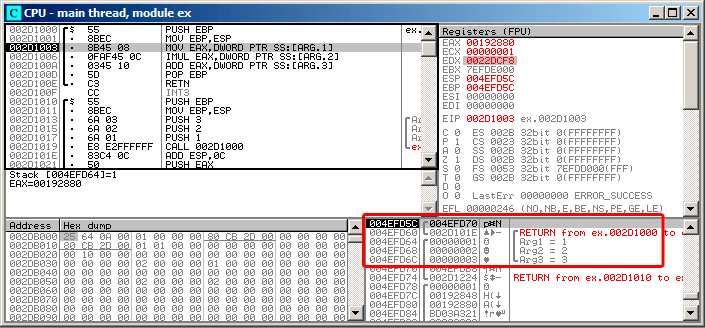
\includegraphics[scale=\FigScale]{patterns/05_passing_arguments/olly.png}
\caption{\olly: внутри функции \ttf{}}
\label{fig:passing_arguments_olly}
\end{figure}
